\documentclass[10pt,a4paper]{report}
\usepackage[latin1]{inputenc}
\usepackage{amsmath}
\usepackage{amsfonts}
\usepackage{color}
\usepackage{amssymb}
\usepackage{graphicx}
\usepackage{fancyhdr}
\lhead{Introduction to \\ Computer Graphics}
\chead{Exercise number}
\rhead{Kevin Serrano, 204141 \\ Gianni Scarnera, 195899}
\pagestyle{fancy}
\author{Kevin Serrano, Gianni Scarnera}
\title{Exercise 3}
\date{24 October 2012}
\begin{document}
\maketitle

\section*{Part 3.2  Transformation and Translation}
First we have to calculate the dimension of the near plane. Given the angle in y-axis from the camera to the near plane and the distance of the near plan, we can calculate the distance of the $top,bottom,left,right$ from the center of the near plane.
\begin{figure}[h!]
\caption{Camera, near plane and far plane}
  \centering
    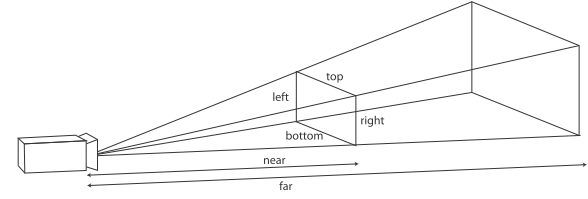
\includegraphics[width=0.7\textwidth]{plane.png}
\end{figure}
\begin{figure}[h!]
\caption{angle}
  \centering
    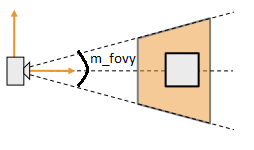
\includegraphics[width=0.5\textwidth]{angle.png}
\end{figure}
Then the half-height is given by trigonometric rule $$half\-height = nearPlane \cdot tan(m_{fovy}/2)$$ where m\_fovy is in degree. Then we can do a ration to figure out the half-width and then $$half\-width = half\-height \cdot Height/Width$$ where Height and Width are from the camera.
Then we can juste compute the $top,bottom,left,right$ as 	$bottom = -half\-eight;
        top = half\-height;
        left = -half\-width;
        right = half\-width;$\\
Then the projection matrix is given in the course and is \[ \left( \begin{array}{cccc}
$$(2 \cdot n)/(r-l)$$ & 0 & $$(r+l)/(r-l)$$ & 0\\
0 & $$(2 \cdot n)/(t-b)$$ & $$(t+b)/(t-b)$$ & 0\\
0 & 0 & $$-(f+n)/(f-n)$$ & $$-(2nf)/(f-n)$$\\
0 & 0 & -1 & 0\end{array} \right)\] 
Then in the cube.vs file, we applied the transformation in this order to get the gl\_position :
$$gl_{Position} = (ProjectionMatrix * WorldCameraTransform * ModelWorldTransform) * gl_{Vertex};$$
\newpage

The translation matrix is given in the course: 
\[ \left( \begin{array}{cccc}
1 & 0 & 0 & t_x\\
0 & 1 & 0 & t_y\\
0 & 0 & 1 & t_z\\
0 & 0 & 0 & 1\end{array} \right)\] 
so we can return this matrix in $getTranslationMatrix()$

Now the difficulty to implement the $translateWorld()$ and $translateObject()$ functions is that we have to do the multiplication in correct order, because matrices multiplication isn't ever commutative as we've seen in lecture.
For $translateWorld()$, the translation must be applied after all previous matrices and it's the inverse for $translateObject()$, i.e :
for $translateWorld()$
$$m\_transformationMatrix = getTranslationMatrix(\_trans) \cdot m\_transformationMatrix;$$
and for $translateObject()$
$$m\_transformationMatrix = m\_transformationMatrix \cdot getTranslationMatrix(\_trans);$$
where $m\_transformationMatrix$ is the current transformation matrix.
\end{document}